% !TeX root = RJwrapper.tex
\title{boundHTS: A R package for coherent hierarchical forecasting of bounded outcomes}


\author{by Hannah Comiskey, David Frazier, and Ole Maneesoonthorn}

\maketitle

\abstract{%
An abstract of less than 150 words.
}

\section{Introduction}\label{introduction}

A hierarchical time series is a multivariate time series subject to linear aggregation constraints \citep{Hyndman2022}. Forecasts for such series are considered coherent when lower-level predictions aggregate exactly to higher levels, satisfying the system's aggregation constraints. In practice, base forecasts are often produced independently at each level, which can lead to incoherence. Forecast reconciliation provides a principled post-processing framework that adjusts these base forecasts to produce aggregate-consistent predictions while retaining as much of the original information as possible \citep{Hyndman2021}. Forecasts may be either point forecasts, representing single most-likely future values, or probabilistic forecasts, representing a distribution over possible future outcomes. A comprehensive review of point and probabilistic reconciliation methods is provided by \citet{Athanasopoulos2024}.

Several R packages on CRAN implement forecast reconciliation across diverse scenarios, including point versus probabilistic forecasts, discrete versus continuous data, and different hierarchical structures (e.g., temporal or cross-sectional). While forecast reconciliation has been studied extensively for discrete and continuous-valued time series, comparatively little attention has been given to hierarchical forecasting under bounded constraints.

One of the most widely used packages for point-forecast reconciliation of hierarchical and grouped time series is \CRANpkg{hts} \citep{htspackage}. This package implements classical methods such as bottom-up (BU), where bottom-level forecasts are aggregated to form higher-level predictions, and top-down (TD), where parent-level forecasts are disaggregated to child nodes. It also provides more advanced methods, including the Optimal Combination (OC) approach of \citet{Hyndman2011} and the Minimum Trace (MinT) method of \citet{Wickramasuriya2019}. OC uses a regression-based framework to adjust forecasts at the bottom level so that they aggregate coherently, while MinT formulates reconciliation as a constrained optimization problem that minimizes the trace of the reconciled forecast error covariance matrix. The \CRANpkg{fabletools} package extends hierarchical reconciliation to the tidyverse ecosystem, providing BU, TD, middle-out (MO), and MinT methods \citep{fabletools}. Both \CRANpkg{hts} and \CRANpkg{fabletools} focus on point forecasts for cross-sectional hierarchies, assuming underlying Gaussian distributions. For more complex or non-standard structures, including temporal hierarchies, \CRANpkg{FoReco} offers flexible reconciliation methods with efficient sparse matrix handling, though it also targets point forecasts only \citep{FoReco}.

For probabilistic reconciliation, the works of \citet{Taieb2017} and \citet{Panagiotelis2023} have been foundational. The \CRANpkg{ProbReco} package explicitly frames reconciliation as an optimization problem based on proper scoring rules, generating coherent probabilistic samples by minimizing the Energy Score \citep{gneiting2007, Panagiotelis2023, ProbReco}. However like the aforementioned packages, this method also only considers reconciliation of data generated from Gaussian distributions. Many empirical applications further involve discrete or bounded supports, introducing additional challenges that are not adequately addressed by these standard Gaussian-based reconciliation methods. \CRANpkg{bayesRecon} enforces coherence through conditioning under aggregation constraints. It supports Gaussian data as well as count data, employing Bottom-Up Importance Sampling (BUIS) to produce lower-bounded, aggregate-consistent probabilistic forecasts \citep{Corani2023, bayesRecon}. However, this package does not deal with fully-bounded distributions like the Beta distribution for the reconciliation of proportions.

To address these challenges, we present the \pkg{boundHTS} package which generates coherent hierarchical forecasts for bounded continuous and lower-bounded discrete variables. Our contribution lies in providing a method to obtain coherent and accurate forecast densities for both bounded and lower-bounded densities. The approach respects the natural bounds of parent distributions. We demonstrate its performance using simulated Beta and Poisson hierarchical data structures.

\section{\texorpdfstring{Theory and Methods unpinning \pkg{boundHTS}}{Theory and Methods unpinning }}\label{theory-and-methods-unpinning}

\section{\texorpdfstring{Using \pkg{boundHTS}}{Using }}\label{using}

\subsection{Case 1: Aggregating count forecasts}\label{case-1-aggregating-count-forecasts}

\subsubsection{The data}\label{the-data}

To begin, we consider a two-tier cross-sectional hierarchical time series where the observations are simulated from low-count Poisson distributions. The hierarchical structure is given by Figure @ref(fig:sim\_poisson\_setup). We consider a scenario where four bottom series (M=4) and 2000 observations (N=2000). The rate parameters of the bottom series are generated using generalised linear models with a log-link. These rate parameters then generate low-value counts via the Poisson distribution. Additional variability is introduced to the bottom series counts using integer values shocks to each series to perturb these series subject to a strict non-negativity constraint. To generate the top-level series, the rate parameters of the bottom series are aggregated. The complete procedure for the data simulation procedure can be found in the Supplementary Materials. This simulated data is stored as \texttt{poisson\_sim\_data} within \pkg{boundHTS}. To evaluate the utility of our method, we split the data into 1750 training observations and 250 test observations.

\begin{figure}
\centering
\pandocbounded{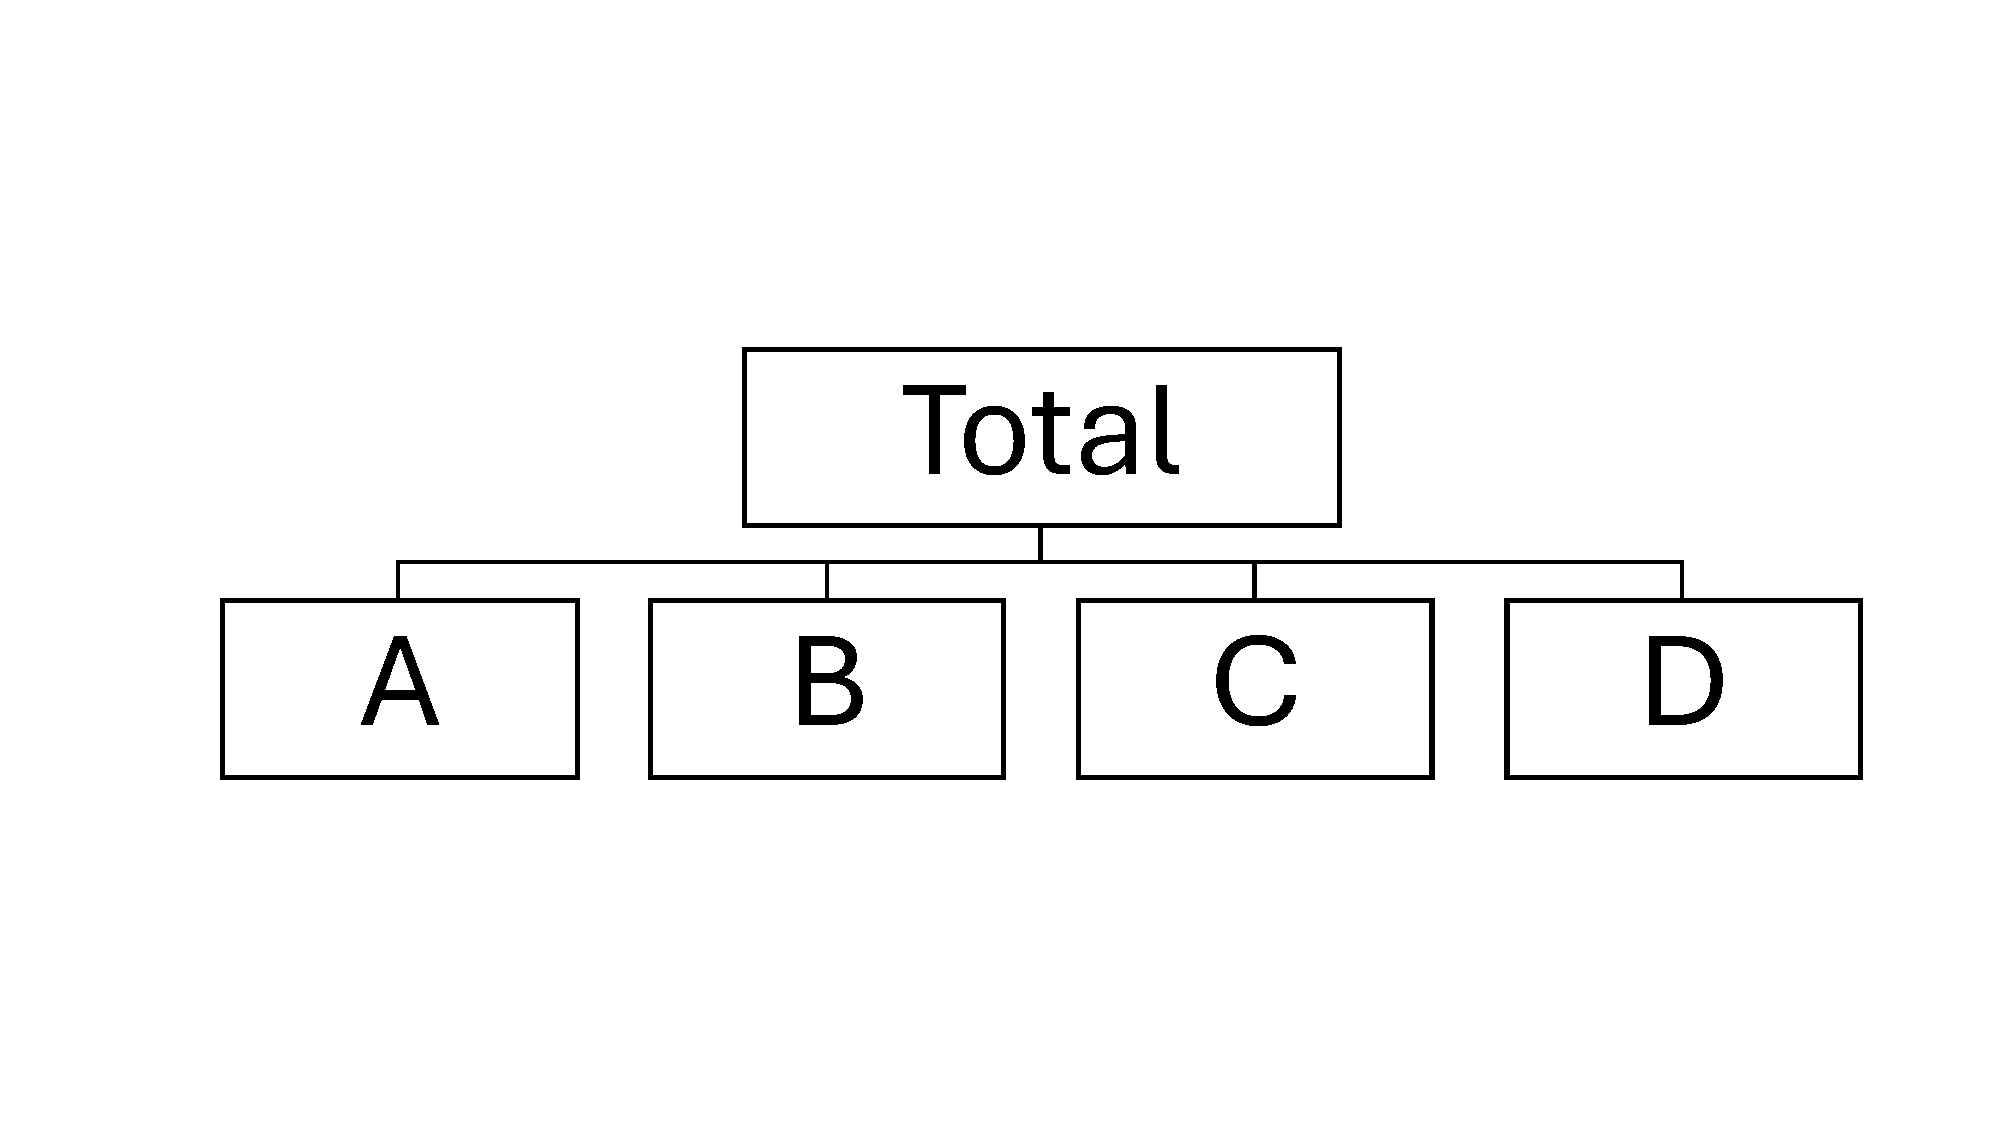
\includegraphics[keepaspectratio]{figures/sim_node_hierarchy.pdf}}
\caption{(\#fig:sim\_poisson\_setup)The two-level hierarchical set up of the Poisson simulation. The four child nodes (A, B, C, D) aggregate to the parent node, Total.}
\end{figure}

\subsubsection{Modelling the base forecasts}\label{modelling-the-base-forecasts}

To obtain base forecasts, we fit standard generalized linear models (GLMs) independently to each node in the hierarchy using \texttt{glm()} from the \pkg{stats} package. These models serve as a simple and reproducible forecasting baseline; our primary contribution lies in the reconciliation methodology applied to the resulting forecasts. For each node, we generate a series of rolling one-step-ahead forecasts. At each step, we record both the in-sample fitted values and the one-step-ahead predictive mean for the rate parameter of each observation. These values are subsequently used to construct a predictive point forecast for each series. These predictions form the base point forecasts that are subsequently reconciled.

\subsubsection{Coherent hierarchical forecasting}\label{coherent-hierarchical-forecasting}

We construct a coherent probabilistic forecast for the top-level series by combining bottom-level Poisson forecasts through convolution and subsequently enforcing moment consistency via exponential tilting. As the sum of independent Poisson random variables is also Poisson, we may use a stepwise procedure in which lower-level tilted densities are convolved to form the starting density of their parent node. This ensures that the resulting probability mass function (PMF) respects aggregation constraints while aligning with the predictive means obtained from the base models.

The procedure requires:

\begin{itemize}
\tightlist
\item
  Predictive mean estimates for the top-level series (\texttt{A})
\item
  Predictive mean estimates for the bottom-level series (\texttt{AA}, \texttt{AB}, \texttt{BA}, \texttt{BB})
\item
  A discrete support grid over which the PMFs are evaluated
\end{itemize}

To begin, we assume the bottom series is given by \(b_{m, t} \sim \mathrm{Poisson}(\lambda_{m,t})\) and let the mean of these forecasts be given by \(\hat{\lambda}_{m,t}\). Taking advantage of the summation property of Poisson distributed variables, the expected value of the convoluted top series density is given by \(\sum_{i=1}^{j}\lambda_{i,t}\). Thus via convolution, the estimated PMF of the top series node is given by,
\begin{align}
    f_{m+1,t}(u_{t}) &=
    \frac{ (\sum_{i=1}^{j}\lambda_{i,t})^{u_{t}} e^{-(\sum_{i=1}^{j}\lambda_{i,t})}}{u_{t}!},
    \qquad u_{t} \in \mathbb{N}_0.
\end{align}

For illustration, base forecasts are generated using a rolling Poisson GLM. The implementation is provided in a helper function within the article for reproducibility, but the reconciliation framework is model-agnostic and can be applied to any suitable base forecasts.

\begin{verbatim}
N <- nrow(boundHTS::poisson_sim_data) 
test_indices  <- seq(from = N - 49, to = N)

glm_results <- rolling_poisson_glm(sim_data = poisson_sim_data,
                                   test_indices =  c(N-49):N,
                                   series_names = c("Tot", "AA", "AB", "BA", "BB"))
\end{verbatim}

To reconcile the mean of the convolution and the predictive mean \(\hat{\lambda}_{k,t}\), we apply exponential tilting using the estimated tilting parameter and predictive means of each series.

\begin{verbatim}
bottom_series <- c("AA", "AB", "BA", "BB")
top_y_vals <- seq(from = 0, to = max(poisson_sim_data$Tot)+10)
n_support <- length(top_y_vals)
n_series  <- length(bottom_series) + 1  # top + bottom

f_tilde_exp <- vector("list", length(test_indices))
nu_exp      <- vector("list", length(test_indices))

for (i in seq_along(test_indices)) {

  t_idx <- test_indices[i]

  # Extract predictive means at time t
  lambda_mat <- glm_results$lambda[[i]]
  lambda_t   <- lambda_mat[t_idx, ]

  lambda_bottom <- lambda_t[bottom_series]
  
  # convolution of bottom series
  lambda_top    <- sum(lambda_bottom) 
  lambda_vec <- c(Total = lambda_top, lambda_bottom)

  ## Allocate storage
  f_tilt <- matrix(0, nrow = n_support, ncol = n_series)
  nu_vec <- numeric(n_series)

  # Construct tilted PMFs
  for (k in seq_along(lambda_vec)) {
    
    # Get PMF of convoluted top series
    base_pmf <- stats::dpois(top_y_vals, lambda_vec[k])
    
    # Find tilting parameter
    nu_k <- stats::uniroot(
      moment_condition_tilting,
      interval  = c(-1, 1),
      f_y       = base_pmf,
      y_vals    = top_y_vals,
      mu_theory = lambda_t[k]
    )$root
    
    # Save tilting parameter
    nu_vec[k] <- nu_k
        
    # Tilt convoluted density towards predictive mean of top series
    f_tilt[, k] <- tilted_density_discrete(
      nu = nu_k,
      f_y = base_pmf,
      y_vals = top_y_vals
    )
  }

  colnames(f_tilt) <- names(lambda_vec)

  f_tilde_exp[[i]] <- f_tilt
  nu_exp[[i]]      <- nu_vec
}
\end{verbatim}

Figure \citet{ref}(fig:poisson-tilted-plot) displays the exponentially tilted predictive mass functions for the top and bottom level series at a representative forecast origin. The unadjusted Poisson distribution implied by aggregation is shifted via exponential tilting so that its expected value coincides with the predictive mean from the base model. As expected, the adjustment primarily alters the tail behaviour of the distribution while maintaining the aggregation constraint.

\pandocbounded{\includegraphics[keepaspectratio]{boundHTS_files/figure-latex/poisson-tilted-plot-1.pdf}}

\subsection{Case 2: Aggregating proportional forecasts}\label{case-2-aggregating-proportional-forecasts}

\section{Appendix}\label{appendix}

\subsection{Data generating process for Poisson data of Case 1}\label{data-generating-process-for-poisson-data-of-case-1}

The bottom-level series are constructed using a generalized linear model with a quadratic log-link. For each series \(m=1,\dots,M\), regression coefficients are drawn independently from a uniform distribution,
\begin{align*}
(\theta_{0,m}, \theta_{1,m}, \theta_{2,m}) \sim \text{Uniform}(0.4,\,0.5).
\end{align*}
A common covariate \(x_{t}\) is drawn for each observation \(t=1,\dots,N\) from a uniform distribution on \([0,1]\),
\begin{align*}
x_{t} \sim \text{Uniform}(0, 1).
\end{align*}
The Poisson rate parameter is then defined as
\begin{align*}
\lambda_{m,t} &= \exp\!\big( \theta_{0,m} + \theta_{1,m}x_t + \theta_{2,m} x_t^2 \big),
\end{align*}
with observed counts generated according to
\begin{align*}
b_{m,t} &\sim \text{Poisson}(\lambda_{m,t}).
\end{align*}
To introduce additional variability, integer-valued shocks
\(\varepsilon_{m,t} \in \{-1,0,1\}\) are added independently to each \(b_{m,t}\).
The distribution of \(\varepsilon_{i,m}\) is series-specific to ensure that noise does not systematically cancel out when aggregating across series:
\begin{align*}
\begin{aligned}
\varepsilon_{1,t} &\sim \{-1,0,1\} \;\; \text{with probabilities } (0.3,0.4,0.3), \\
\varepsilon_{2,t} &\sim \{-1,0,1\} \;\; \text{with probabilities } (0.5,0.4,0.1), \\
\varepsilon_{3,} &\sim \{-1,0,1\} \;\; \text{with probabilities } (0.33,0.33,0.34), \\
\varepsilon_{4,t} &\sim \{-1,0,1\} \;\; \text{with probabilities } (0.2,0.3,0.5).
\end{aligned}
\end{align*}
To ensuring non-negativity, the perturbed bottom-level series are then given by
\begin{align*}
b^{*}_{m,t} = \max\!\big(0,\, b_{m,t} + \varepsilon_{m,t}\big).
\end{align*}\\
At the aggregate level, the series is obtained by summing across the unperturbed bottom-level counts:
\begin{align*}
y^\text{tot.}_t  = \sum_{m=1}^M b_{m,t}.
\end{align*}
The final noisy dataset consists of 2000 draws of the covariate \(x\), the aggregate series \(\text{Tot}\), and the four perturbed bottom-level series \((b^{\ast}_{1},\dots,b^{\ast}_{4})\).

\bibliography{RJreferences.bib}

\address{%
Hannah Comiskey\\
Monash Univeristy\\%
Department of Econcometrics and Business Statistics\\ Melbourne, Australia\\
%
\url{https://hannahcomiskey.github.io/}\\%
\textit{ORCiD: \href{https://orcid.org/0000-0003-0034-6725}{0000-0003-0034-6725}}\\%
\href{mailto:hannahcomiskey@monash.edu}{\nolinkurl{hannahcomiskey@monash.edu}}%
}

\address{%
David Frazier\\
Monash Univeristy\\%
Department of Econcometrics and Business Statistics\\ Melbourne, Australia\\
%
%
%
%
}

\address{%
Ole Maneesoonthorn\\
Monash Univeristy\\%
Department of Econcometrics and Business Statistics\\ Melbourne, Australia\\
%
%
%
%
}
